\documentclass[journal]{IEEEtran}

% Additional packages
\usepackage{graphicx}
\usepackage{amsmath}
\usepackage{hyperref}
\usepackage{float}
\usepackage{subcaption}
\usepackage{booktabs}
\usepackage{pgfplotstable}
\usepackage{qrcode}

\pgfplotsset{compat=1.18}

\begin{document}
 
\title{Analysis of RLC Circuits: Serial and Parallel Configurations}
\author{IBRAHIM H.I. ABUSHAWISH \\
Istanbul University, Department of Physics \\
Instructor: Res. Asst. Öznur ARSLAN \\
Experiment Date: 6.12.2024, Report Submission Date: 16.12.2024\\
Course \& Section Number: PHYS2305}

\maketitle

\begin{abstract}
    This report presents a comprehensive analysis of RLC circuits, including serial and parallel configurations. It provides a detailed theoretical overview, experimental procedures, data analysis, and discussion of key findings. The analysis is supported by code-based calculations and graphical visualizations produced using Python. Key conclusions indicate that resonance frequency shifts are primarily determined by capacitance in fixed resistance scenarios, while resistance impacts peak sharpness and impedance values. Experimental results revealed resonance peaks at approximately 230 Hz for the parallel RLC circuit with fixed capacitance and 200 Hz for the series RLC circuit with fixed capacitance. Practical implications include the design of frequency filters and oscillators based on RLC circuit configurations.
\end{abstract}
    
\section{Introduction}
RLC circuits are fundamental in the study of alternating current (AC) electrical systems. They serve as essential components in filters, oscillators, and resonant circuits. This report aims to explore the behavior of both serial and parallel RLC circuits. Key objectives include analyzing the resonance phenomenon, calculating impedance, and visualizing phase shifts. The study emphasizes how resistance, capacitance, and inductance interact under varying frequencies.

\section{Theory}

\subsection{Serial RLC Circuit}
A serial RLC circuit consists of a resistor (R), inductor (L), and capacitor (C) connected in series. The voltage applied across the circuit can be described as:
\begin{equation}
    U(t) = IR + L\frac{dI(t)}{dt} + \frac{Q}{C}
\end{equation}
where $U(t)$ is the applied voltage, $I(t)$ is the current, $R$ is the resistance, $L$ is the inductance, $C$ is the capacitance, and $Q$ is the charge on the capacitor. Solving for impedance $Z$, the following expression is obtained:
\begin{equation}
    Z = \sqrt{R^2 + \left(\omega L - \frac{1}{\omega C}\right)^2}
\end{equation}
The resonance frequency $f_0$ occurs when the impedance is minimal and is calculated as:
\begin{equation}
    f_0 = \frac{1}{2\pi \sqrt{LC}}
\end{equation}
At resonance, the current is maximum, and the circuit appears purely resistive.

\subsection{Parallel RLC Circuit}
A parallel RLC circuit has R, L, and C elements connected in parallel. The total impedance $Z$ is calculated as:
\begin{equation}
    \frac{1}{Z} = \frac{1}{j\omega L} + j\omega C + \frac{1}{R}
\end{equation}
The condition for resonance in a parallel RLC circuit is when the reactive components cancel each other, leading to:
\begin{equation}
    \omega_0 = \frac{1}{\sqrt{LC}}
\end{equation}
The quality factor, bandwidth, and impedance characteristics of parallel RLC circuits are analyzed to identify the conditions for maximum energy transfer.

\section{Experimental Setup}
The experimental setup~\ref{fig:experimental_setup} involves several essential components, including resistors, capacitors, and inductors, which are connected to form serial and parallel RLC circuits. An AC power source is used to provide alternating current, and measurements are taken using the Cobra3 PowerGraph software. The circuit diagrams for both serial and parallel RLC circuits are illustrated in Figures \ref{fig:serial_circuit} and \ref{fig:parallel_circuit}, respectively.

\begin{figure}[H]
    \centering
    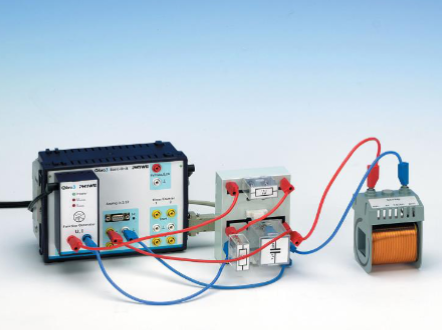
\includegraphics[width=\linewidth]{IMAGES/Experimental_setup.png}
    \caption{Circuit elements and experimental setup.}
    \label{fig:experimental_setup}
\end{figure}

\begin{figure}[H]
    \centering
    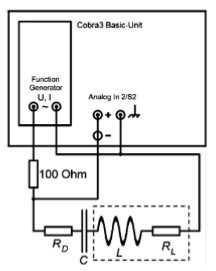
\includegraphics[width=0.5\linewidth]{IMAGES/series_diagram.png}
    \caption{Circuit diagram of a Serial RLC circuit.}
    \label{fig:serial_circuit}
\end{figure}

\begin{figure}[H]
    \centering
    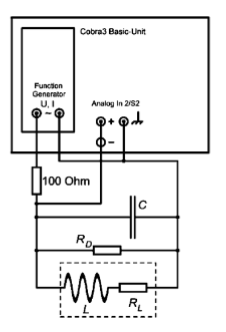
\includegraphics[width=0.5\linewidth]{IMAGES/parallel_diagram.png}
    \caption{Circuit diagram of a Parallel RLC circuit.}
    \label{fig:parallel_circuit}
\end{figure}

\section{Experimental Procedure}
The experiment began by configuring the RLC circuit components as per the schematic diagrams for both serial and parallel configurations. Each component, including resistors, capacitors, and inductors, was connected appropriately, and the AC power source was attached to provide the required alternating current. The Cobra3 PowerGraph software was used to monitor the circuit's response in real time.

For the fixed capacitance analysis, the capacitance value was set to 2.2 µF for both serial and parallel configurations. The resistance was then varied, and measurements of the impedance and resonance frequencies were recorded for each resistance value. This process allowed for the observation of the impact of resistance on the resonance behavior of the RLC circuits.

In the fixed resistance analysis, the resistance was set to 220 ohms, and the capacitance was varied for both the serial and parallel configurations. Measurements of the impedance and resonance frequencies were recorded for capacitance values of 1 µF, 2.2 µF, and 4.7 µF. This part of the procedure highlighted the impact of capacitance on the resonance frequency of the circuits.

The recorded data for all measurements was saved for subsequent analysis. Impedance vs. frequency graphs were plotted for the fixed capacitance and fixed resistance configurations. These visualizations provided a clear representation of the resonance peaks and shifts in impedance, aiding in the analysis and discussion of the RLC circuit behavior.


\section{Results}

\subsection{Raw Data}
Raw data is available in the GitHub repository \cite{github}, in \verb|10th_Experiment_RLC/DATA/|.

\subsection{Configurations and Notation}
Table \ref{tab:configurations} provides the naming conventions used in the graphs and their corresponding configurations.

\begin{table}[H]
    \centering
    \caption{Configurations and Notations Used in Graphs}
    \label{tab:configurations}
    \begin{tabular}{cccc}
    \toprule
    \textbf{Notation} & \textbf{Configuration} & \textbf{Capacitance µF} &  \textbf{Resistance $\Omega$} \\
    \midrule
    P\_22c\_220R  & Parallel & 2.2 &220\\
    P\_22c\_470R  & Parallel & 2.2 &470\\
    P\_22c\_680R  & Parallel & 2.2 &680\\
    S\_22c\_220R  & Series & 2.2 &220\\
    S\_22c\_470R  & Series & 2.2 &470\\
    S\_22c\_680R  & Series & 2.2 &680\\
    P\_1c\_220R   & Parallel & 1 &220\\
    P\_47c\_220R  & Parallel & 4.7 &220\\
    S\_1c\_220R   & Series & 1 &220\\
    S\_47c\_220R  & Series & 4.7 &220\\
    \bottomrule
    \end{tabular}
\end{table}
\subsection{Graphical Analysis}
The following figures illustrate the relationship between impedance and frequency for both RLC circuit types, analyzed for fixed capacitance and resistance values. Key resonance peaks are identified and labeled in the graphs.

\begin{figure}[H]
    \centering
    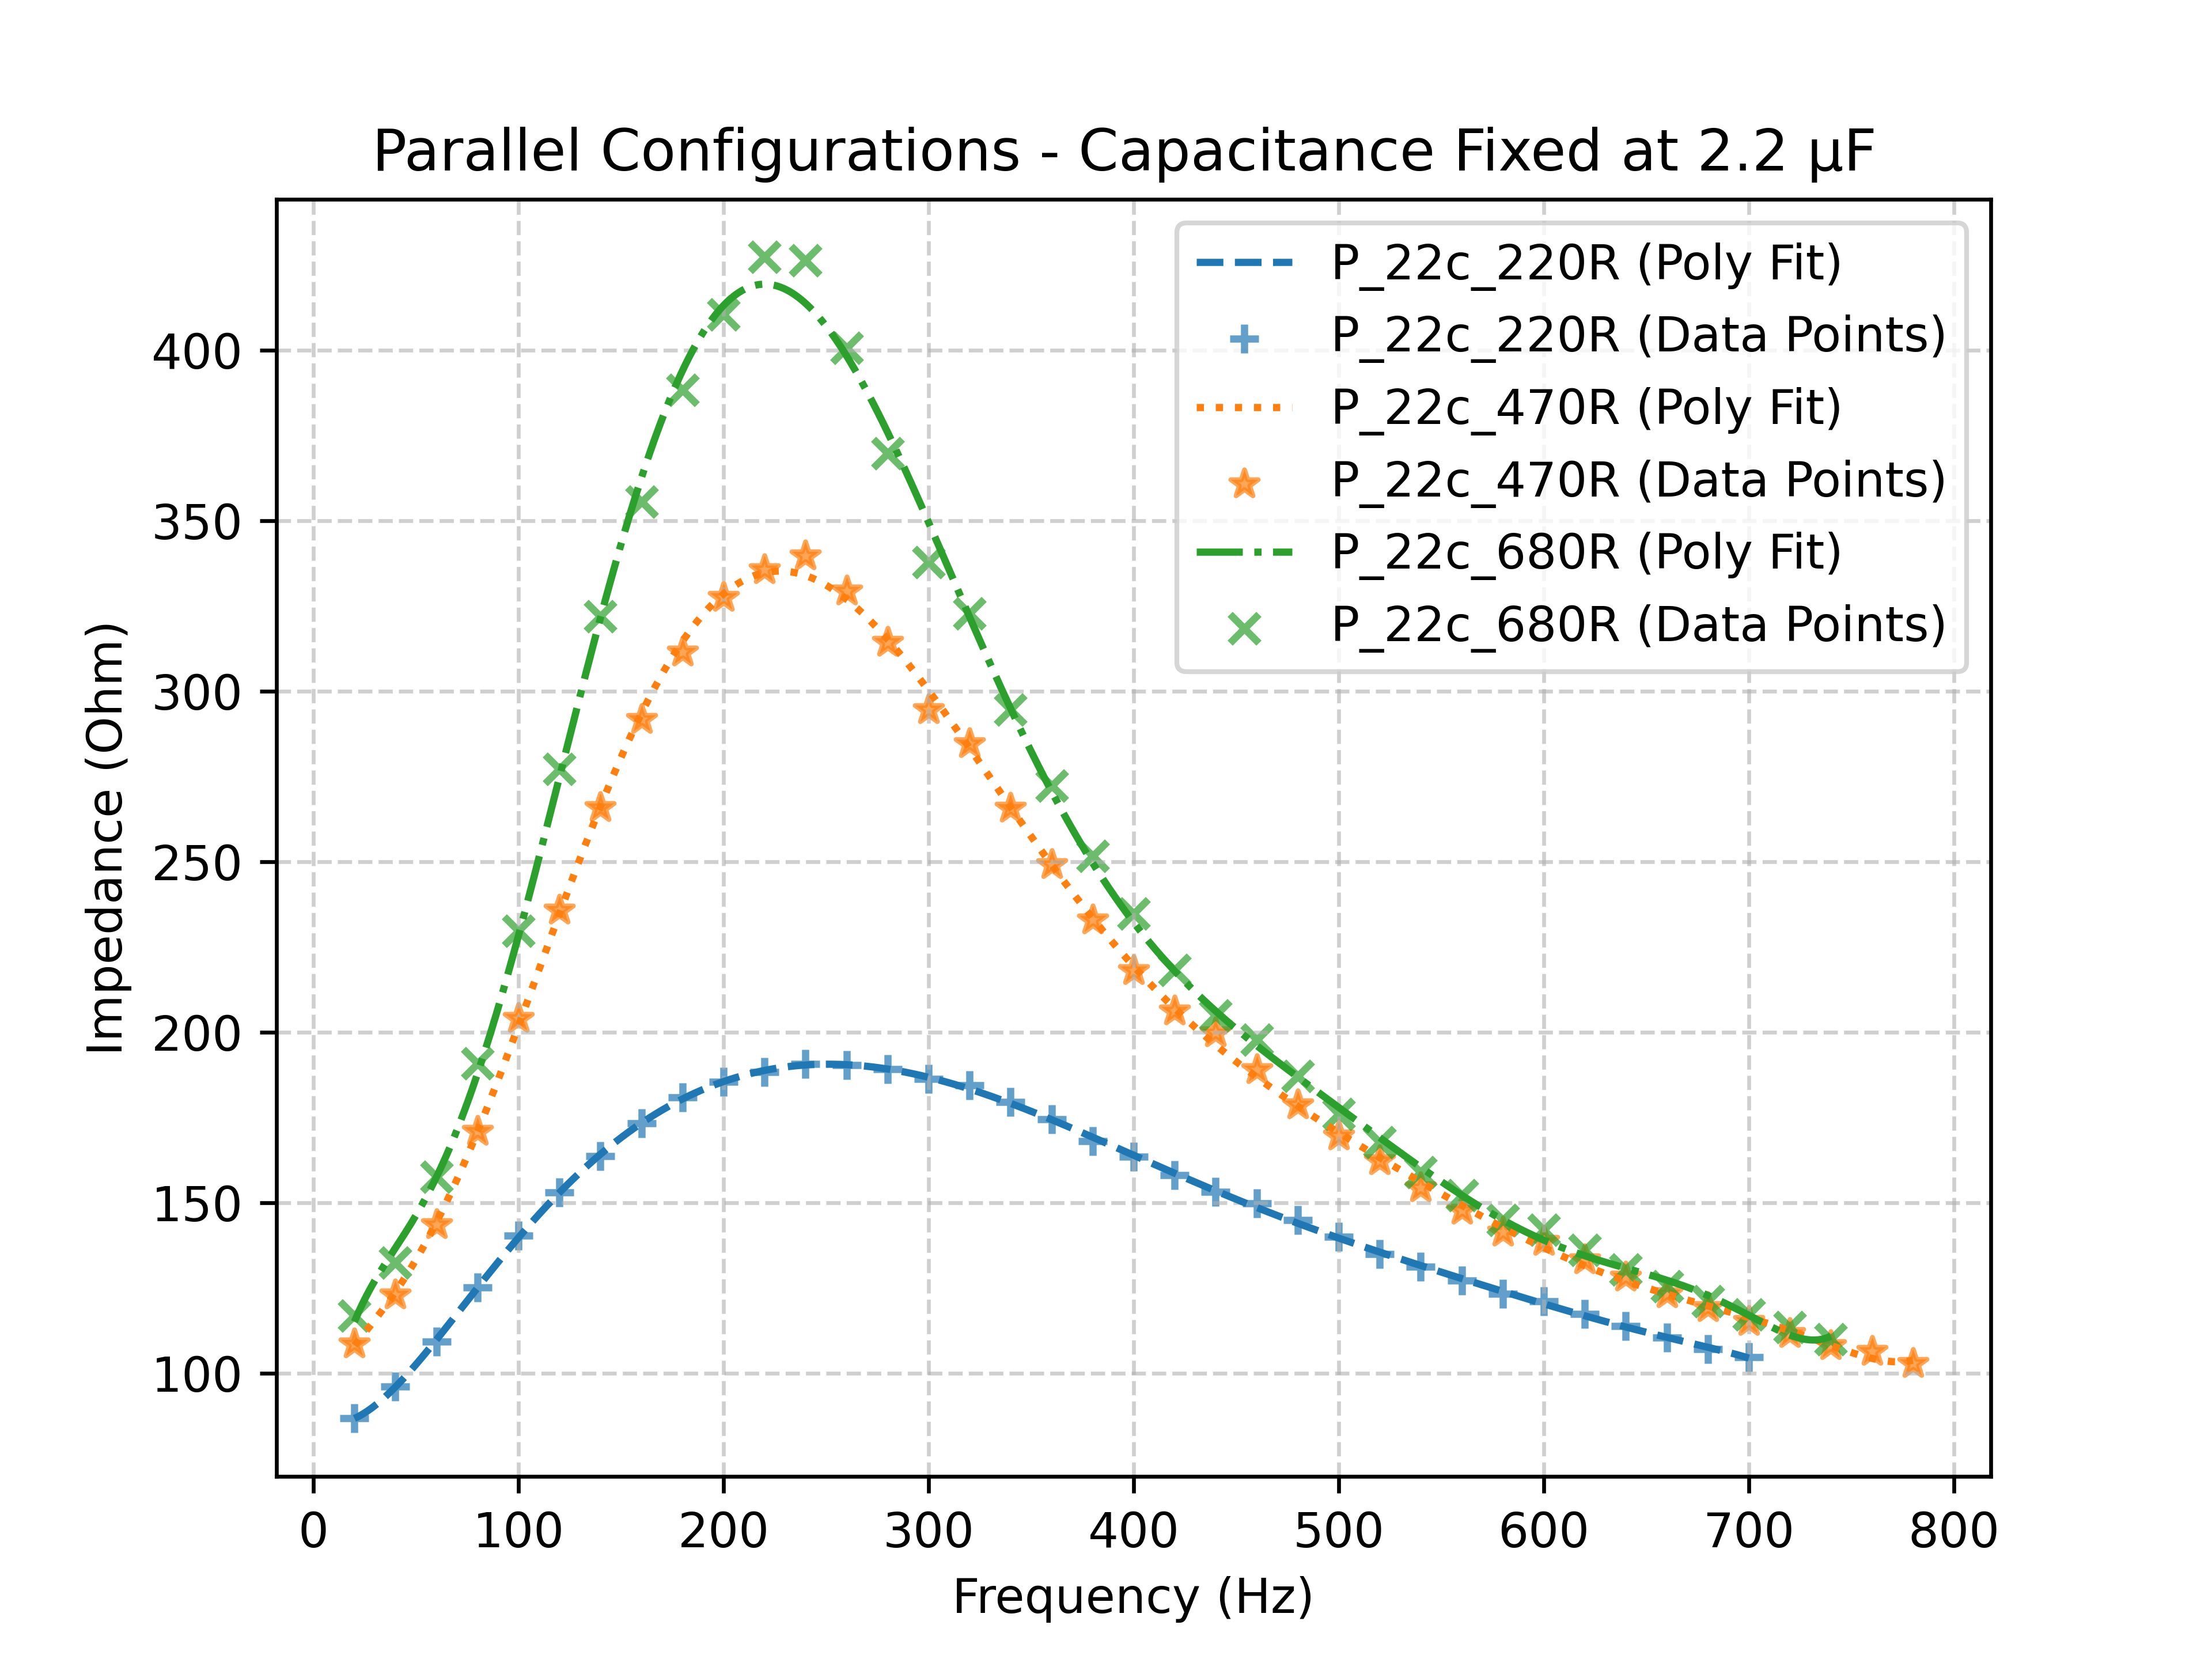
\includegraphics[width=\linewidth]{output_plots/Fixed_C/Parallel.png}
    \caption{Parallel RLC circuit with fixed capacitance. The resonance peak is observed at approximately 230 Hz.}
    \label{fig:parallel_fixed_c}
\end{figure}

\begin{figure}[H]
    \centering
    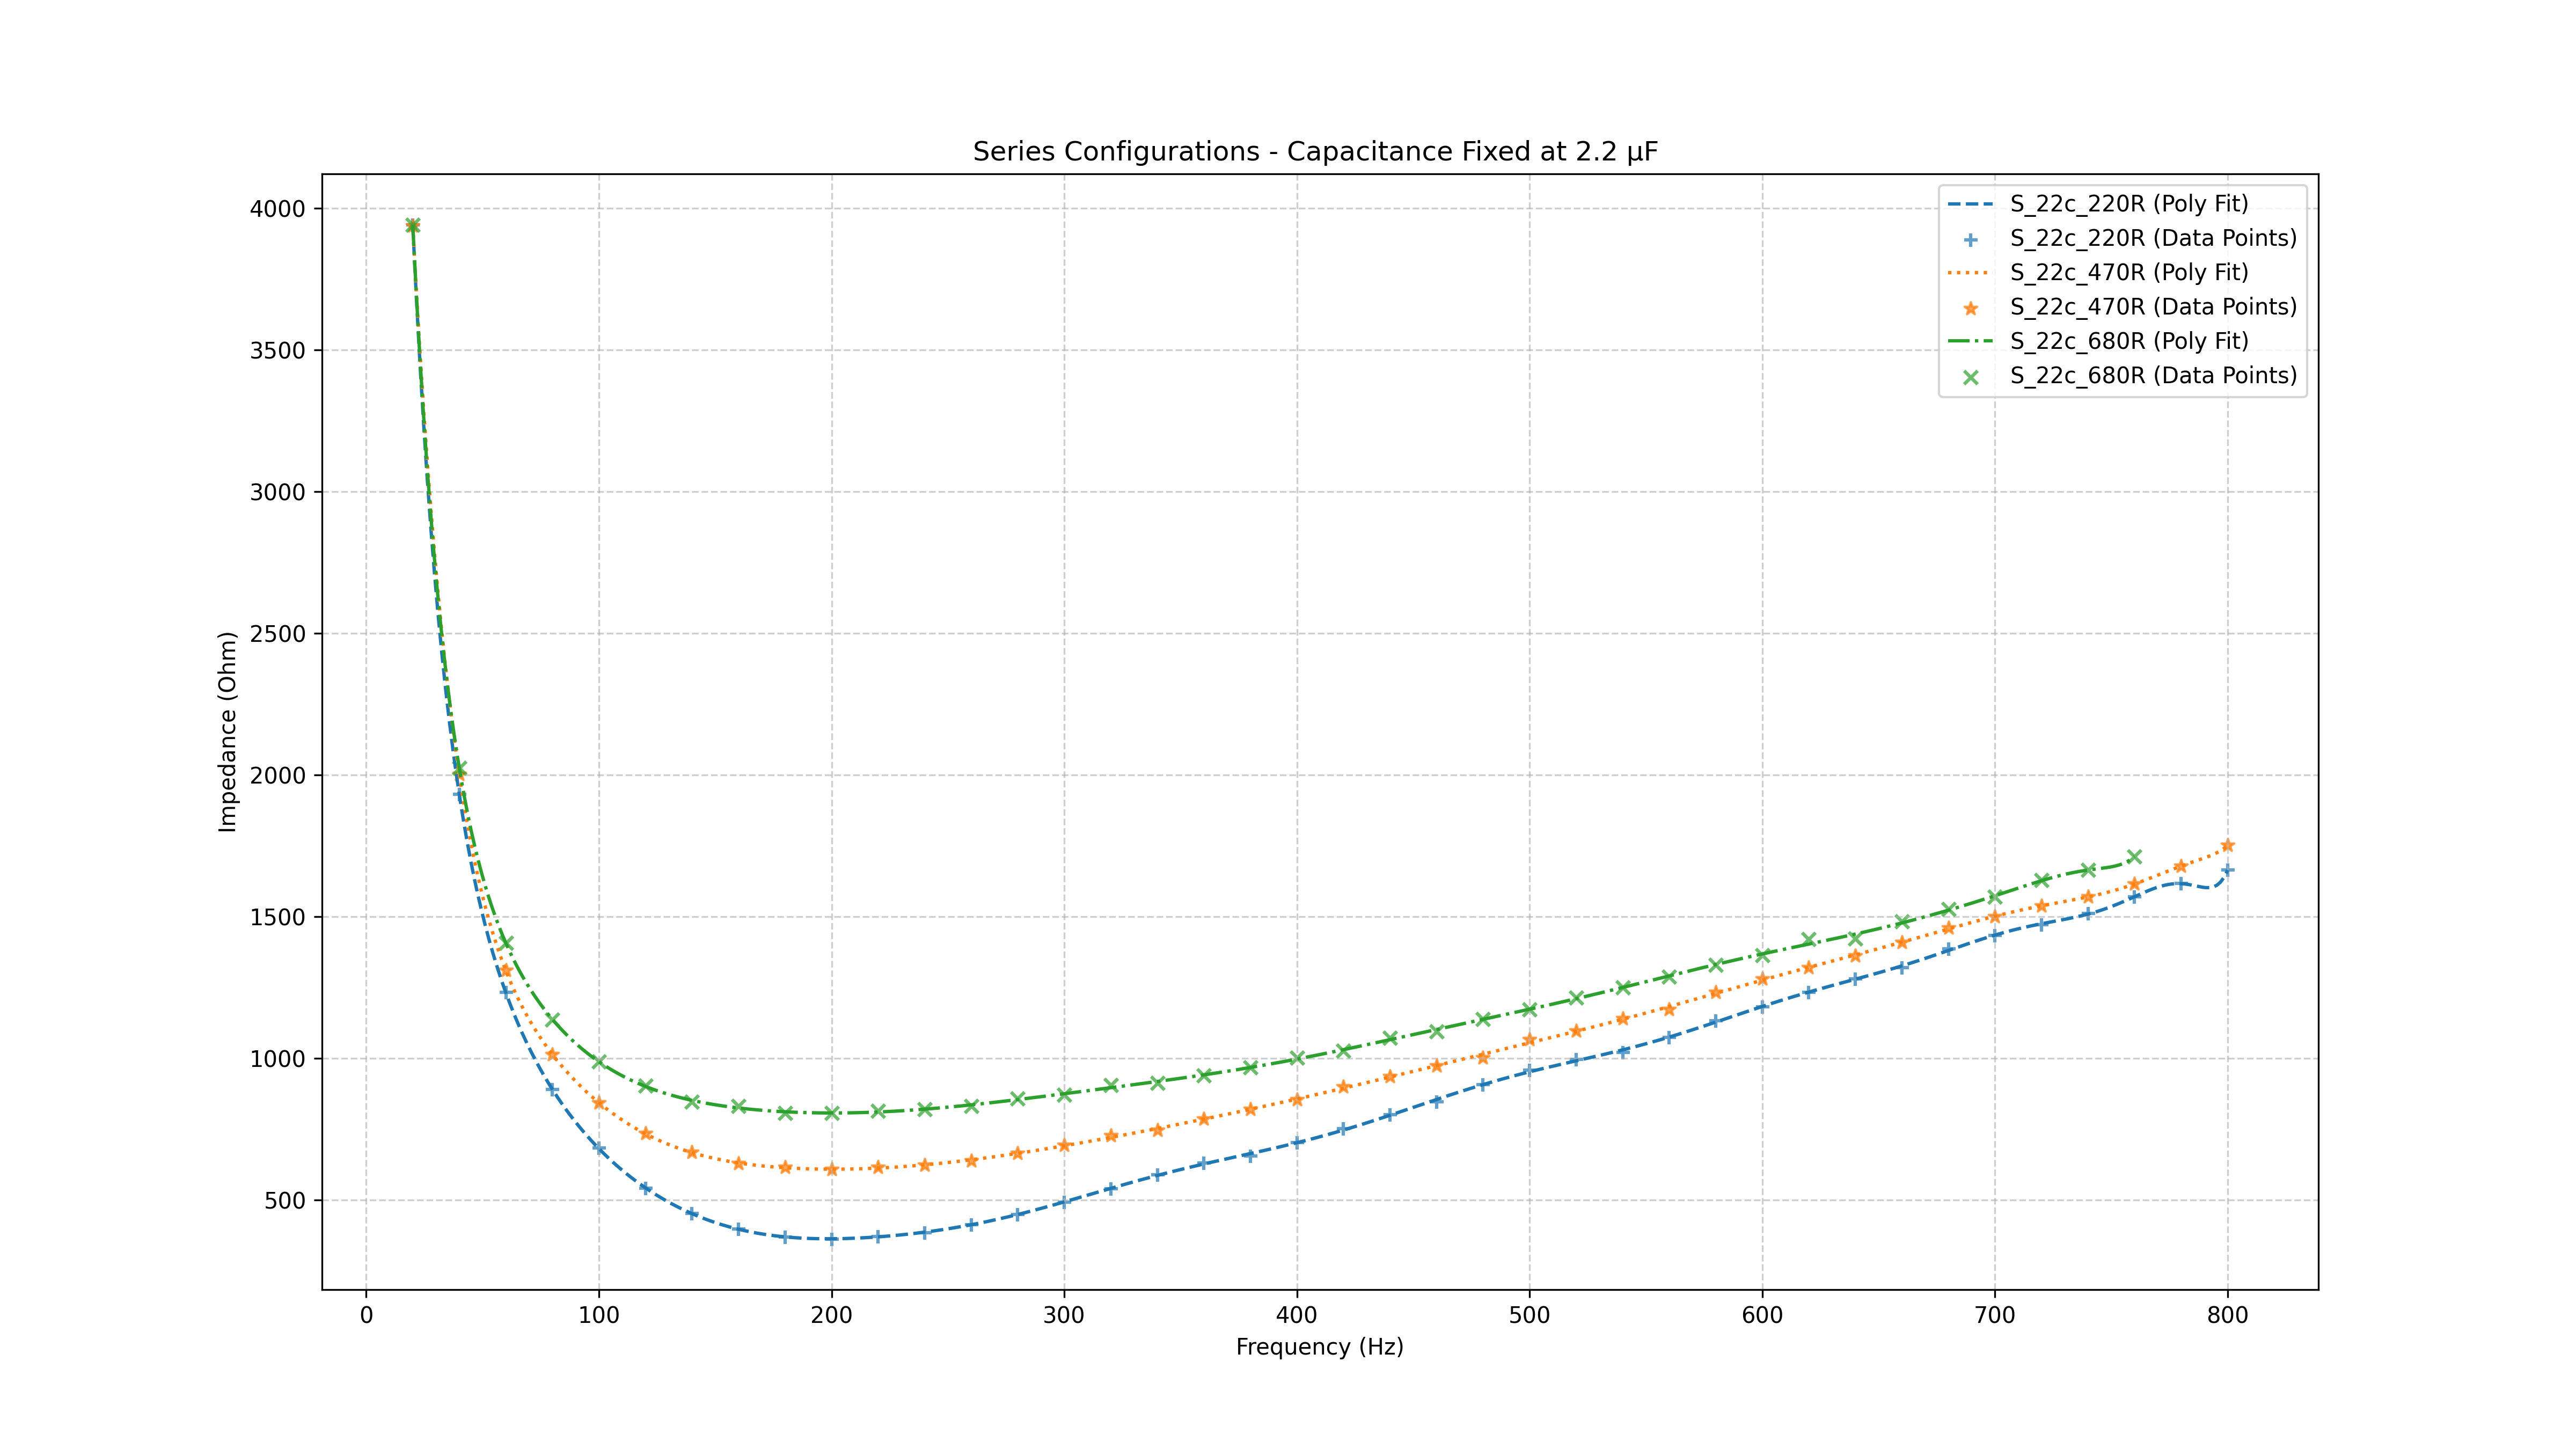
\includegraphics[width=\linewidth]{output_plots/Fixed_C/Series.png}
    \caption{Serial RLC circuit with fixed capacitance. The resonance peak is observed at approximately 200 Hz.}
    \label{fig:series_fixed_c}
\end{figure}

\begin{figure}[H]
    \centering
    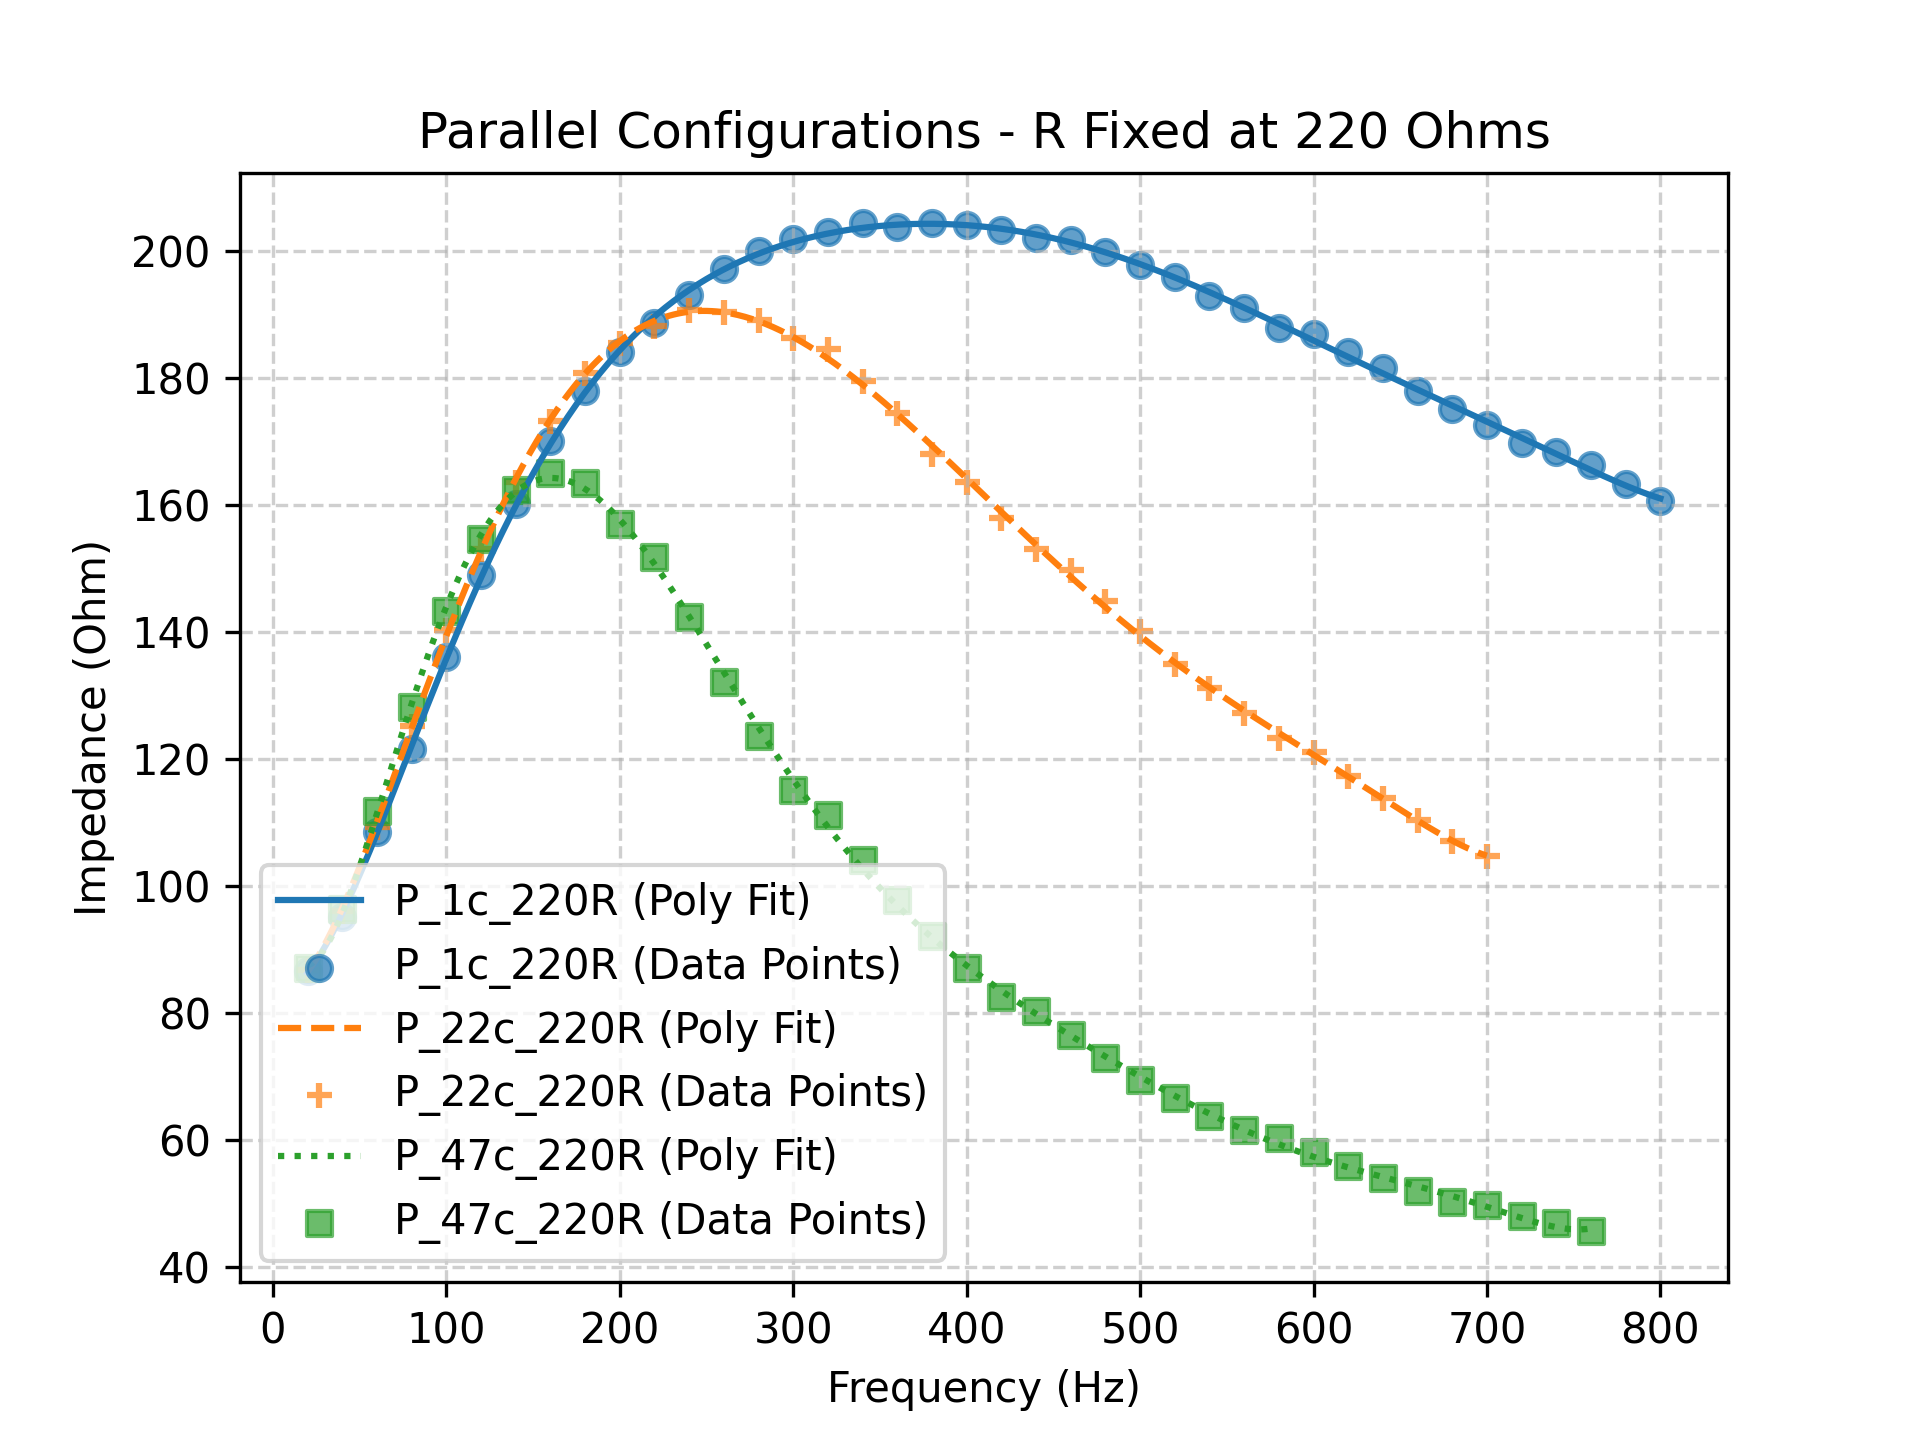
\includegraphics[width=\linewidth]{output_plots/Fixed_R/Parallel.png}
    \caption{Parallel RLC circuit with fixed resistance. The resonance peaks are observed at approximately 150 Hz, 250 Hz, and 350 Hz for 4.7 µF, 2.2 µF, and 1 µF capacitance, respectively.}
    \label{fig:parallel_fixed_r}
\end{figure}

\begin{figure}[H]
    \centering
    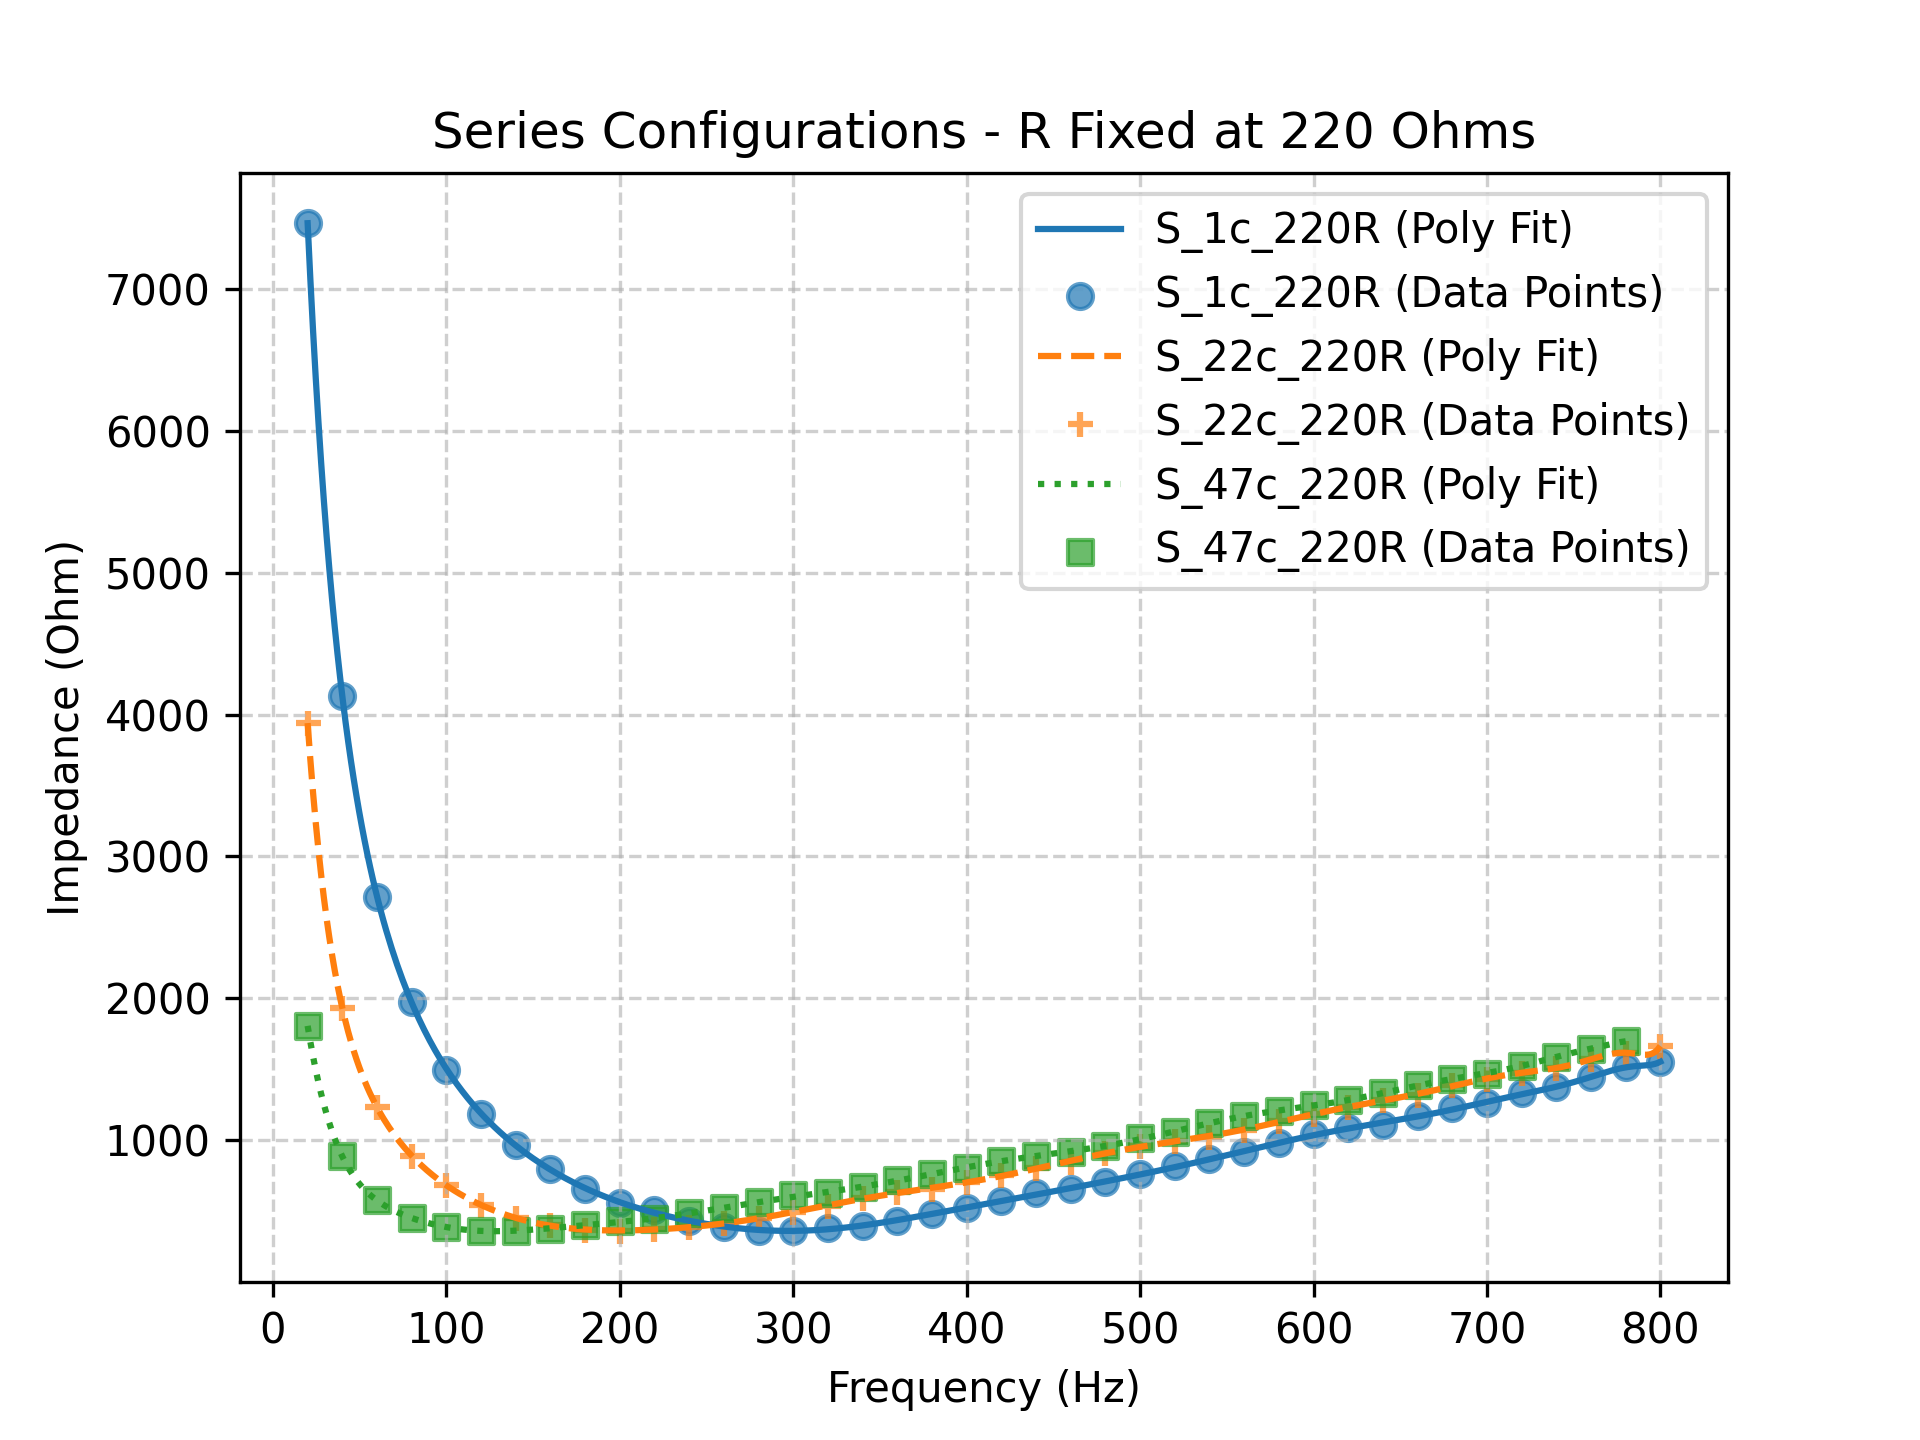
\includegraphics[width=\linewidth]{output_plots/Fixed_R/Series.png}
    \caption{Serial RLC circuit with fixed resistance. The resonance peaks are observed at approximately 100 Hz, 200 Hz, and 300 Hz for 4.7 µF, 2.2 µF, and 1 µF capacitance, respectively.}
    \label{fig:series_fixed_r}
\end{figure}


\section{Discussion}
\subsection{Horizontal Shifts}
\textbf{Fixed Resistance, Variable Capacitance:} In Figures \ref{fig:parallel_fixed_r} and \ref{fig:series_fixed_r}, resonance frequency shifts horizontally due to the dependence on capacitance: \(f_0 = \frac{1}{2\pi\sqrt{LC}}\). Increasing capacitance lowers resonance frequency by increasing the effective reactive impedance.

\textbf{Fixed Capacitance, Variable Resistance:} In Figures \ref{fig:parallel_fixed_c} and \ref{fig:series_fixed_c}, resonance frequency remains constant. However, the sharpness of the resonance peaks is heavily impacted, as resistance directly influences the quality factor \(Q\).

\subsection{Vertical Shifts}
\textbf{Parallel Configurations:} Vertical shifts are pronounced in parallel circuits (Figure \ref{fig:parallel_fixed_c}) as impedance at resonance is inversely proportional to resistance. Higher resistance results in sharper peaks and higher impedance.

\textbf{Series Configurations:} Vertical shifts in series circuits (Figure \ref{fig:series_fixed_c}) show increased minimum impedance values with higher resistance, as impedance at resonance aligns with the resistive component of the circuit.

\subsection{Quality Factor Analysis}
The quality factor \(Q\) determines the sharpness of resonance. Higher \(Q\) values are observed for lower resistance in series circuits, reflecting minimal energy dissipation. Conversely, in parallel circuits, the quality factor improves with increased resistance due to enhanced impedance.

\subsection{Practical Implications}
These behaviors have significant implications for designing filters and oscillators. For example, in communication systems, parallel RLC circuits with high \(Q\) values are used to isolate specific frequency bands, while series circuits are often employed in impedance matching.

\section{Conclusion}
This experiment provides a comprehensive understanding of RLC circuit behavior, emphasizing the effects of varying resistance and capacitance on resonance. From the discussion, it is evident that resonance frequency shifts are primarily determined by capacitance in fixed resistance scenarios, while resistance impacts peak sharpness and impedance values. Practical insights into designing efficient AC circuit components were highlighted.

\section{Additional Resources}
For detailed information, including the Lab Manual, source code, and related experiments, visit the GitHub repository provided below or scan the QR code in Fig.~\ref{fig:qr_code}.

\begin{figure}[H]
    
    \centering
    \begin{minipage}{0.15\textwidth}
        \centering
        \qrcode[height=2cm]{https://github.com/ibeuler/LAB-Reports}
    \end{minipage}%
    \begin{minipage}{0.2\textwidth}
        \raggedright
        \caption{Access the GitHub repository for the lab manual, source code, and related experiments: \href{https://github.com/ibeuler/LAB-Reports}{\url{https://github.com/ibeuler/LAB-Reports}}.}
        \label{fig:qr_code}
    \end{minipage}
\end{figure}

\begin{thebibliography}{9}
\bibitem{lab_manual}
    ISTANBUL UNIVERSITY, \textit{Physics Laboratory II Experiment Book: Electricity and Magnetism}, Department of Physics, 2024.

\bibitem{github}
    \textit{Source code and additional experiments are available in the GitHub repository.} \url{https://github.com/ibeuler/LAB-Reports}
\end{thebibliography}

\end{document}
